\section{Introdução}

Este trabalho prático tem como objetivo a implementação de um analisador léxico e um analisador sintático \textbf{LALR}(\textit{Look-ahead left-to-right}), ambos partes indispensáveis do \textit{front end} de um compilador. 

Para auxiliar a implementação foram utilizadas duas ferramentas escritas em Java: \textbf{JFlex}(\textit{Java Fast Lexical Analyzer Generator}) para gerar o analisador léxico e \textbf{CUP}(\textit{Construction of Useful Parsers}) para gerar o analisador sintático LALR.

As análises devem ser feitas baseadas na gramática apresentada na figura 1.

\begin{figure}[ht]	
 \centering
  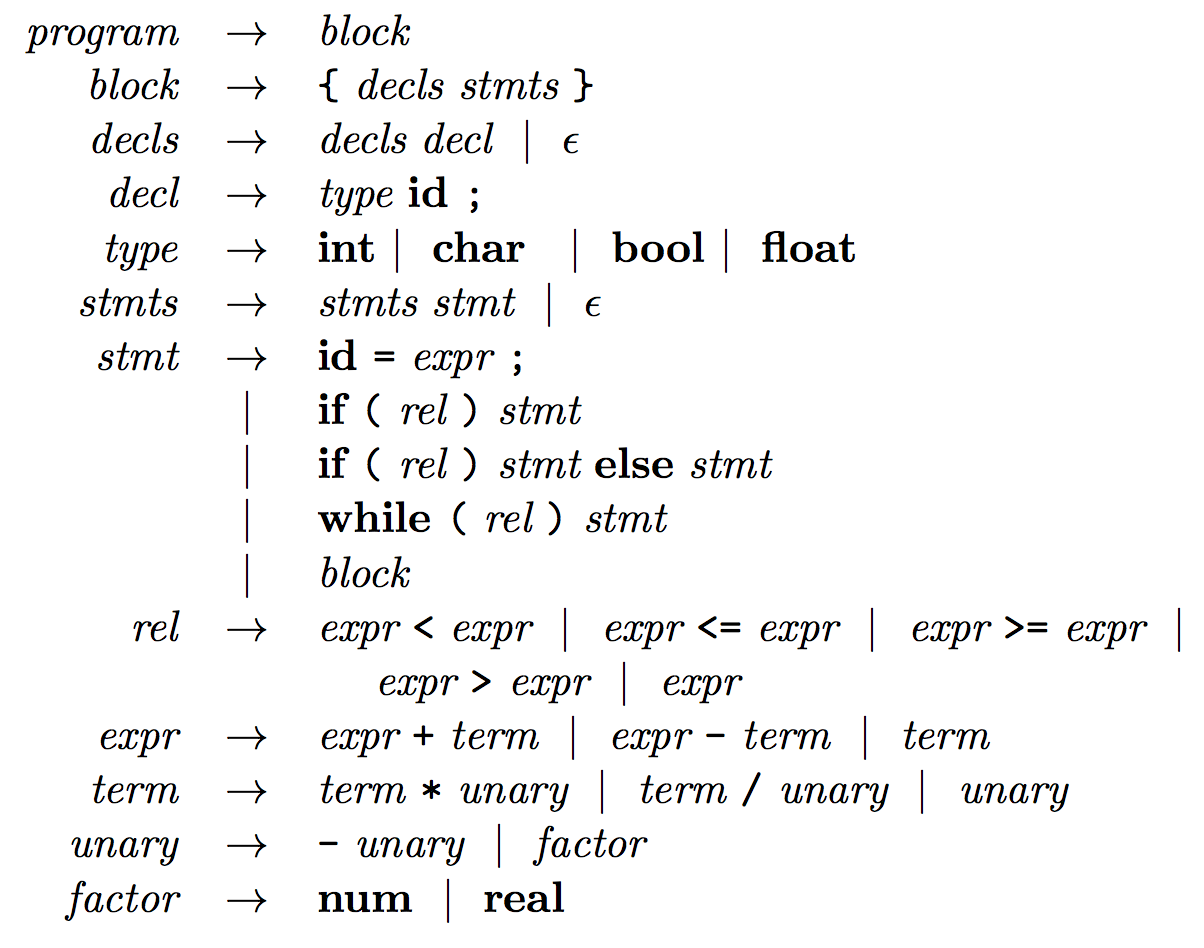
\includegraphics[width=10cm,keepaspectratio]{images/grammar.png}
 \caption{Gramática descrita no enunciado do trabalho.}
\end{figure}
